\documentclass[11pt]{article}
\usepackage{amsmath, amssymb}
\usepackage{geometry}
\usepackage{hyperref}
\usepackage{graphicx}
\usepackage{booktabs}
\geometry{margin=2.5cm}
\graphicspath{{../plots/}}

\newcommand{\ket}[1]{|#1\rangle}
\newcommand{\bra}[1]{\langle#1|}
\newcommand{\Pop}{\hat{P}}
\newcommand{\expv}[1]{\langle #1\rangle}
\newcommand{\Oedge}{X_0 Z_1\cdots Z_{L-2} X_{L-1}}

\title{Is fermion parity protected by topology under noise,\\
and how does the chain length $L$ matter?}
\author{Seminar notes (Block 4 -- the professor's questions)}
\date{\today}

\begin{document}
\maketitle

\begin{abstract}
The professor asked whether the fermion parity of the Kitaev-chain simulation is
``protected by topology,'' and how the chain length $L$ enters. We answer both in
the noisy setting built in Week 9, applying Qiskit's single-qubit decoherence
channels to the topological ground state. The short answers: (Q1) what is
conserved is conserved by \emph{symmetry}, not topology --- phase damping keeps
$\expv{\Pop}$ exactly fixed because it is parity-preserving, while the genuinely
topological object, the non-local edge string, is not noise-immune at any fixed
$L$; (Q2) the chain length acts in \emph{opposite} directions --- the intrinsic
parity gap is protected exponentially, $\Delta_P(L)\sim e^{-L/\xi}$, but the
vulnerability to $T_1$ poisoning and to depolarizing contrast loss \emph{grows}
with $L$.
\end{abstract}

\section{Background: symmetry versus topology}

Under Jordan--Wigner the Kitaev chain is
\begin{equation}
  H = -\frac{\mu}{2}\sum_{j} Z_j
      + \frac{t-\Delta}{2}\sum_j X_j X_{j+1}
      + \frac{t+\Delta}{2}\sum_j Y_j Y_{j+1},
  \qquad
  \Pop = \prod_{j} Z_j .
\end{equation}
Every term has an even number of $X/Y$ factors, so $[H,\Pop]=0$ in \emph{every}
phase: parity conservation is a $\mathbb{Z}_2$ symmetry of the Hamiltonian, not a
topological effect. What topology adds is that in the topological phase
($|\mu|<2t$) the two Majorana ends fuse into one non-local fermion
$f=\tfrac12(\gamma_L+i\gamma_R)$ whose occupation is the parity bit; the even/odd
ground states become degenerate with splitting (the \emph{parity gap})
\begin{equation}
  \Delta_P(L)=\bigl|E_0^{+}-E_0^{-}\bigr|
  \;\approx\; 2t\Bigl(\tfrac{|\mu|}{2t}\Bigr)^{L}=2t\,e^{-L/\xi},
  \qquad \xi^{-1}=\ln\tfrac{2t}{|\mu|}.
\end{equation}
Because $f$ joins the two ends, no \emph{local} operator can read or flip the
bit. The question for Block 4 is what survives once the device decoheres.

\section{Which noise channels respect parity}

A single-qubit channel matters for $\Pop$ only through how its Kraus operators
commute with the local $Z_j$. Using Qiskit's standard channels:
\begin{center}
\begin{tabular}{lccl}
\toprule
Channel (Qiskit) & Acts through & vs.\ $\Pop=\prod_j Z_j$ & Effect on $\expv{\Pop}$\\
\midrule
\texttt{phase\_damping\_error} ($T_2$) & $Z_j$ & commutes (preserving) & exactly conserved\\
\texttt{depolarizing\_error} & $X_j,Y_j,Z_j$ & $X,Y$ anticommute & shrinks $(1-p)^L$ toward $0$\\
\texttt{amplitude\_damping\_error} ($T_1$) & $\sigma^-_j$ & violating, biased to $\ket0$ & leaks to odd sector\\
\bottomrule
\end{tabular}
\end{center}
$Z_j$ commutes with $\Pop$, so dephasing leaves $\expv{\Pop}$ untouched. $X_j,Y_j$
and the lowering operator $\sigma^-=\tfrac{X+iY}{2}$ anticommute with $Z_j$, so a
single such event flips the global parity. Amplitude damping is additionally
\emph{biased}: it preferentially sends $\ket1\to\ket0$, i.e.\ removes
Jordan--Wigner fermions, so it leaks the protected even state into the odd sector
rather than scrambling it symmetrically.

\paragraph{Connection to Week 9.} The realistic \texttt{thermal\_relaxation\_error}
$(T_1,T_2,\tau)$ used in the Week 9 gate-noise study is exactly the composition of
these two pieces: its $T_1$ part is the parity-\emph{violating} amplitude damping,
its $T_2$ part is the parity-\emph{preserving} dephasing. So the two questions
below dissect the same physical channel that drives the circuit-level model.

\section{Q1: is the parity protected by topology, under noise?}

We prepare the exact even-parity ground state at $\mu=t$ (topological), apply each
channel at increasing strength $p$, and read off $\expv{\Pop}$ and the edge string
(Fig.~\ref{fig:parity}). Two different objects behave very differently.
\begin{description}
  \item[The conserved quantity $\expv{\Pop}$ --- protected by \emph{symmetry}.]
    Under phase damping $\expv{\Pop}$ stays \emph{exactly} $1$ (flat to machine
    precision), because the Kraus operators commute with $\Pop$. But this is the
    $\mathbb{Z}_2$ symmetry, which holds in every phase --- it is \emph{not}
    topology. Both parity-violating channels break it: depolarizing drives
    $\expv{\Pop}\to0$ as $(1-p)^L$, and amplitude damping leaks into the odd
    sector ($\expv{\Pop}$ falling, but staying above depolarizing because the
    bias pulls back toward the $\Pop=+1$ vacuum).
  \item[The topological order parameter --- \emph{not} noise-immune.] The
    non-local edge string decays under \emph{every} channel, \emph{including} the
    parity-preserving phase damping that leaves $\expv{\Pop}=1$: dephasing
    destroys the cross-chain coherence the string relies on, so its contrast
    falls even while parity is perfectly conserved.
\end{description}
\textbf{Answer.} Parity conservation is protected against parity-preserving noise
--- but by \emph{symmetry}, not topology --- and is destroyed by parity-violating
noise ($T_1$ poisoning, depolarizing). The genuinely \emph{topological} object,
the non-local edge string, is \emph{not} protected against any noise at fixed
$L$: conserving parity does not preserve the topological signal. Topology does
not buy fixed-$L$ noise immunity; where it enters is the chain-length scaling.

\begin{figure}[h]
  \centering
  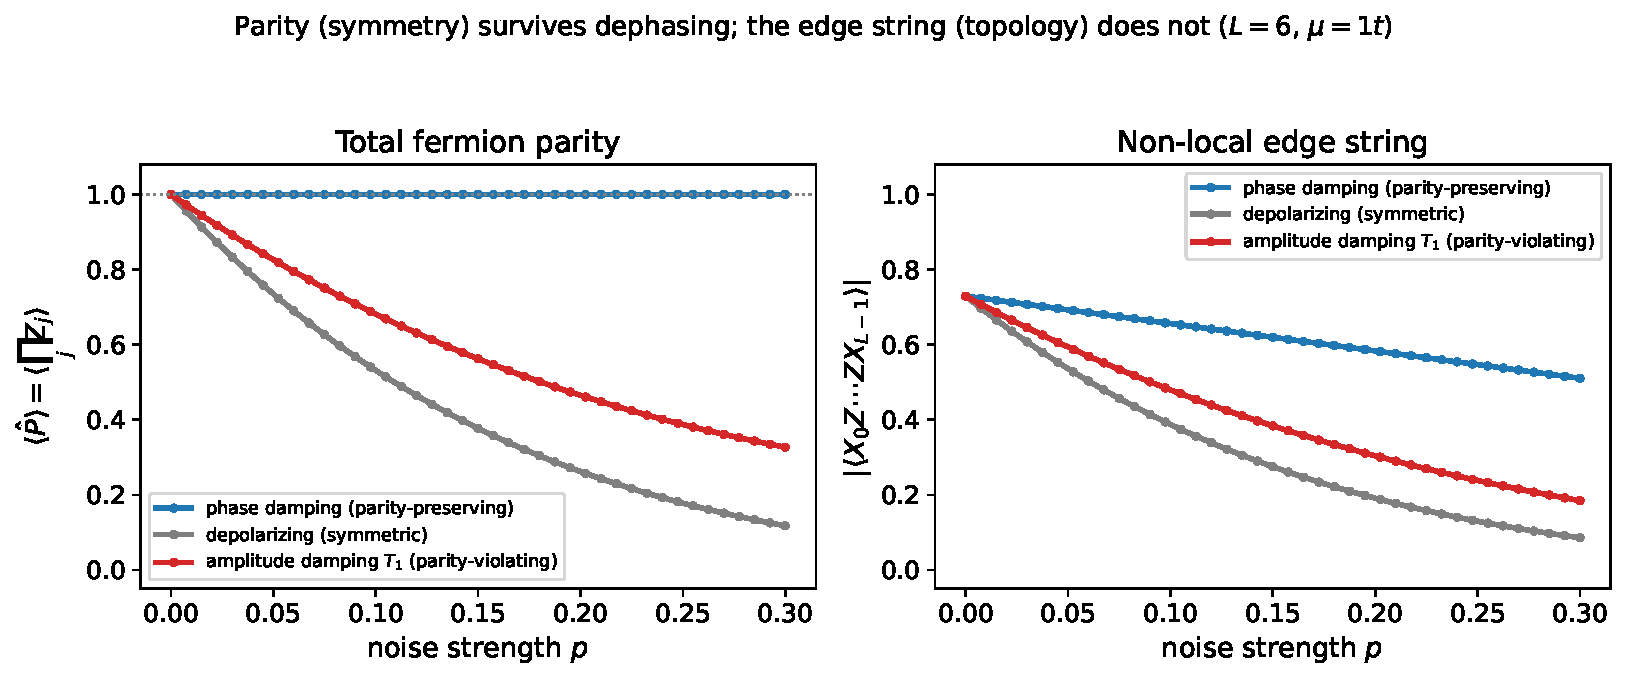
\includegraphics[width=\linewidth]{block4_parity_vs_noise.pdf}
  \caption{Topological state at $L=6$, $\mu=t$, Qiskit single-qubit channels.
  Left: $\expv{\Pop}$ stays exactly $1$ under phase damping (symmetry), collapses
  under depolarizing, and leaks (stays biased high) under amplitude damping.
  Right: the non-local edge string decays under \emph{all} channels --- including
  the parity-preserving phase damping --- so parity conservation does not protect
  the topological signal.}
  \label{fig:parity}
\end{figure}

\section{Q2: how does the chain length change this, under noise?}

Length acts in two competing ways (Fig.~\ref{fig:length}).
\begin{itemize}
  \item \textbf{Intrinsic protection improves with $L$.} Noiselessly,
    $\Delta_P(L)\sim e^{-L/\xi}$ in the topological phase ($\mu=t$): on a semilog
    axis a straight line of slope $\ln(|\mu|/2t)$, falling from $0.41$ at $L=2$ to
    $5.9\times10^{-3}$ at $L=8$. In the trivial phase ($\mu=3t$) the gap is flat
    at $\mathcal{O}(1)$ --- there is no degeneracy to protect.
  \item \textbf{Vulnerability worsens with $L$.} At fixed channel strength
    $\gamma=p=0.1$, the odd-sector leakage under amplitude damping grows from
    $0.03$ to $0.21$ (more sites that can lose a fermion, $\sim1-(1-\gamma)^L$),
    and the edge-string loss under depolarizing grows from $0.19$ to $0.57$ (a
    longer non-local string accumulates more single-qubit contrast loss).
\end{itemize}
\textbf{Answer.} There is no monotone ``longer is better.'' The topological
degeneracy is exponentially better protected at large $L$, but the noisy device
loses parity and contrast faster at large $L$. The two trends oppose, defining an
optimal working length --- the direct analogue, in the chain-length axis, of the
optimal ansatz depth found in Week 9.

\begin{figure}[h]
  \centering
  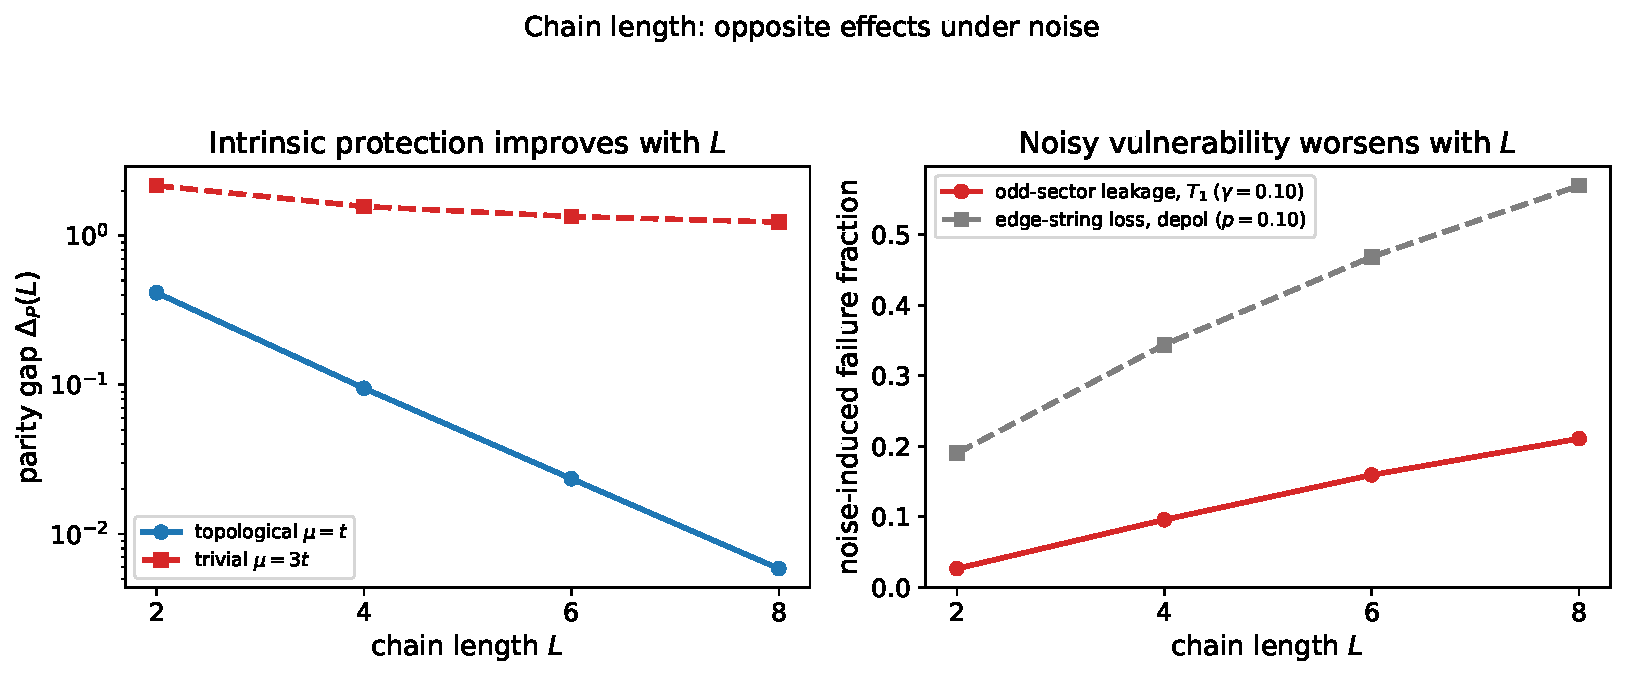
\includegraphics[width=\linewidth]{block4_length_under_noise.pdf}
  \caption{Left: noiseless parity gap $\Delta_P(L)$ --- exponential decay in the
  topological phase (intrinsic protection improving with $L$) versus the flat
  $\mathcal{O}(1)$ trivial gap. Right: at fixed noise $\gamma=p=0.1$, odd-sector
  leakage under $T_1$ and edge-string loss under depolarizing both grow with $L$.
  Longer chains are intrinsically better protected but noisier to operate.}
  \label{fig:length}
\end{figure}

\section{Summary}

\begin{itemize}
  \item Parity \emph{conservation} is a $\mathbb{Z}_2$ symmetry, not topology; it
    survives parity-preserving ($T_2$) noise and is broken by parity-violating
    ($T_1$, depolarizing) noise.
  \item The \emph{topological} object (the non-local edge string / the degeneracy)
    is not noise-immune at fixed $L$ --- every channel erodes it.
  \item Topology's role is in the $L$-scaling: intrinsic protection improves as
    $e^{-L/\xi}$ while the noisy device degrades with $L$, giving an optimal
    length --- the chain-length counterpart of the Week 9 optimal-depth result.
  \item These three axes --- noise strength, ansatz depth (Week 9), and chain
    length --- are the knobs that decide whether a NISQ measurement of the Kitaev
    chain can still resolve the topological phase.
\end{itemize}

\end{document}
